\documentclass[12pt]{article}  % [12pt] option for the benefit of aging markers
\usepackage{amssymb,amsthm}    % amssymb package contains more mathematical symbols
\usepackage{graphicx}          % graphicx package enables you to paste in graphics

\usepackage{tabularx}
\usepackage{setspace}
\usepackage[nottoc,notlot,notlof]{tocbibind}


%%%%%%%%%%%%%%%%%%%%%%%%%%%%%%%%%
%
%    Page size commands.  Don't worry about these
%
\setlength{\textheight}{220mm}
\setlength{\topmargin}{-10mm}
\setlength{\textwidth}{150mm}
\setlength{\oddsidemargin}{0mm}

%%%%%%%%%%%%%%%%%%%%%%%%%%%%%%%%%%%%%%%%%%%%%%%%%%%%%%%%%%%%%%%
%
%    Definitions of environments for theorems etc.
%
\newtheorem{theorem}{Theorem}[section]          % Theorems numbered within sections - eg Theorem 2.1 in Section 2.
\newtheorem{corollary}[theorem]{Corollary}      % Corollaries etc. will be counted as Theorems for numbering
\newtheorem{lemma}[theorem]{Lemma}              % eg Lemma 3.1, ... Theorem 3.2, ... Corollary 3.3.
\newtheorem{proposition}[theorem]{Proposition}
\newtheorem{conjecture}[theorem]{Conjecture}

\theoremstyle{definition}
\newtheorem{definition}[theorem]{Definition}

\theoremstyle{remark}
\newtheorem{remark}[theorem]{Remark}
\newtheorem{example}[theorem]{Example} 
%%%%%%%%%%%%%%%%%%%%%%%%%%%%%%%%%%%%%%%%%%%%%%%
%
%        Preamble material specific to your essay
%
\title{Lab Marking system \\~\\  \large{Heriot-Watt University} \\~\\ Final Year Dissertation}
\author{Lewis McNeill\\
supervised by
Peter J King}

\begin{document}
\maketitle
\pagenumbering{gobble}
\newpage 

\doublespacing
\textbf{\Large{Declaration}} \\[2em]
I, Lewis Francis McNeill, confirm that this work submitted for assessment is my own and is expressed in my own words. Any uses made within it of the works of other authors in any for (e.g., ideas, equations, figures, text, tables, programs) are properly acknowledged at any point of their use. A list of the references employed is included.
\\
\\
Signed: Lewis McNeill
\\
Date: \today

\newpage                    
\begin{abstract}

The project aim is to develop a web application that will be used to improve marking of computing labs. The application will be designed to be used by Students to quickly know their grade, by Lab Helpers to easily mark labs and Lecturers to see marking immedatly as it is done.



\end{abstract}

\newpage                     

\singlespacing
\tableofcontents
\doublespacing



\newpage        

\section{Aims, Objectives and Project Description}
\setcounter{page}{1}
\pagenumbering{arabic}

\subsection{Aim}
The aim of this dissertation is to design and implement a system for the digital marking and analysis of computer labs, to help improve the speed at which they are marked.

And provide statics on how the class is proforming as a whole


\subsection{Objectives}
\begin{itemize}
\item Simplify the way that labs marks are currently processed.
\item Allow lecturers to create marking schemes on-line that lab helps can access and mark students against in labs.
\item Develop a system that allows lab helps to mark labs using an on-line application.
\item Allow students to see the mark they got from the lab instantly.
\item Provide useful statistics and graphs to lecturers.
\end{itemize}






\newpage
\section{Literature Review}

This section contains the current academic literature relating to the digitalisation of marking systems. 
\subsection{Digital Marking Systems}
Digital marking systems are designed to mirror current paper based marking systems but take advantage of the electronic enviroment \cite{joy_effective_1998}

\subsection{User Dependant Views}


\subsection{Data to Graphics}





\newpage
\section{Requirements}
\subsection{System Requirements}


\begin{tabularx}{\textwidth}{|l|X|X|X|X|}
\hline
  \textbf{ID} & \textbf{Requirement} & \textbf{Type} & \textbf{Description} & \textbf{Priority} 
\\
\hline
R1&Test&Test&Test&Test\\ \hline
R2&Test&Test&Test&Test\\ \hline


\end{tabularx}

\subsection{Usability Requirements}







\newpage
\section{Strategy for testing and evaluation}

\subsection{Testing}
Throughout the development of the system, unit tests will be used to make sure that the system is robust and functional. \\

\subsection{Evaluating}
To properly evaluate how successful I have been at creating a new Lab Marking System I will conduct a usability case study. Lecturers, lab helpers and students will be asked to use the systems and provide feed back, to help evaluate the system and discover what improvements can be made to make it better.

Efficency of the code










\newpage
\section{Project Plan and Professional, Legal, Ethical and Social Issues}

\subsection{Project Plan}

The gantt chart for this dissertation can be seen in figure(\ref{fig:ganttchart}). It is broken down into 5 sections: Design, Development, Evalutation, Disertation and Poster.\\
\textbf{Design Stage} Starts at the end of semester 1 to allow myself time to complete other course work. In this stage I will create mock-ups for the user interface, a database schema and define what will be occuring in each of my sprints in the next stage.\\
\textbf{Development Stage:} Starts once the holidays are over. It consists of three two week sprints each it a weeks break inbetween to allow for write ups and other coursework. When the three sprint finishs I go straigh into the evaluation stage.\\ 
\textbf{Evaluation Stage: } on last for two week, in this period I will conduct a useability case study and write up the remainder of my diseration for the draft handin.\\
\textbf{Final Deliverable Stage:} This stage is for me to focus on feedback from the draft hand-in and make sure my Dissertation is of a high enough standard.\\
\textbf{Poster Stage:} This stage entirely dedicated to the design and creation of my disertation poster.

\begin{figure}[!htbp]

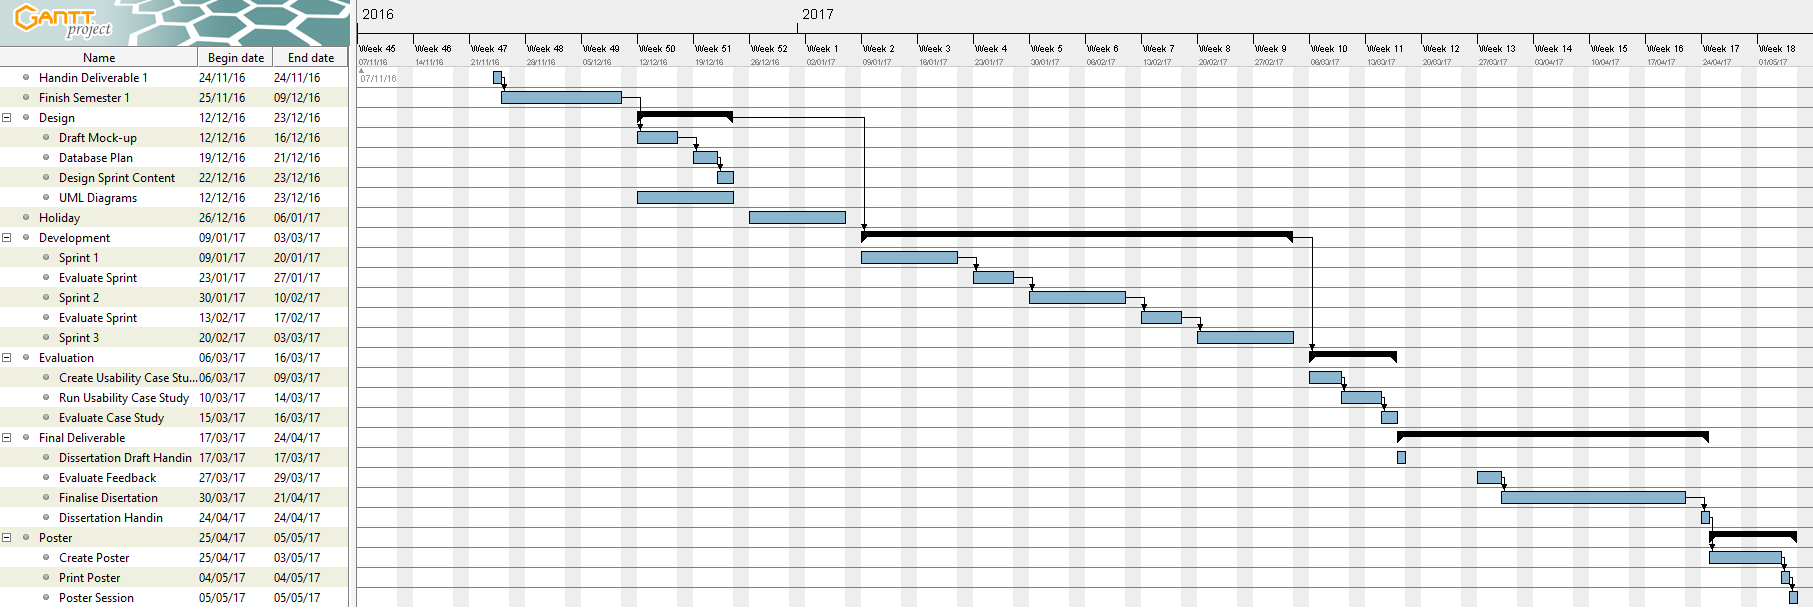
\includegraphics[width=\textwidth]{images/ganttchart.png}
\caption{Project Gantt Chart}
\label{fig:ganttchart}

\end{figure}




\subsection{Risk Analysis}
\newcounter{risk} \stepcounter{risk}
The risk relating to this dissertation are shown in tabel(\ref{table:risk})

\begin{table}[h]
\begin{tabular}{|p{0.05\textwidth}|p{0.5\textwidth}|p{0.22\textwidth}|p{0.22\textwidth}|}


\hline
  \textbf{ID} & \textbf{Risk} & \textbf{Importance} & \textbf{Likelihood }
\\
\hline
R\arabic{risk} &Test&Test&Test\\ \hline \stepcounter{risk}
R\arabic{risk} &Test&Test&Test\\ \hline \stepcounter{risk}
R\arabic{risk} &Test&Test&Test\\ \hline \stepcounter{risk}
R\arabic{risk} &Test&Test&Test\\ \hline \stepcounter{risk}
R\arabic{risk} &Test&Test&Test\\ \hline \stepcounter{risk}
R\arabic{risk} &Test&Test&Test\\ \hline


\end{tabular}

\caption{Risk Analysis}
\label{table:risk}

\end{table}






\subsection{Professional}
 The professional part of this project will be done by following coding standards for the languages that I decide to use.
 As this project will be a Web application I will that both the html and css are validated an

\subsection{Legal}
There are multiple legal issues relating to this project. The most important one is the Data Protection Act, since the systems will be designed to store data about student I will have to make sure that 

\subsection{Ethical}

A major ethical requirement of this project is to do with the storage of students personal information on a digital system. Is it ethical to keep all 

no decieving see their own marks

\subsection{Social}

A few social issues are raised by this project. Such as if students can see the mark they have recieved straight away, will this result in markers raising grades to try and not offend the students.

Will this system result in a reduction of lab helps being required to mark labs. If the system speeds up the time to mark students less lab helps may-be need to run labs, resulting in people looking work.



%%%%%%%%%%%%%%%%%%%%%%%%%%%%%%%%%%%%%%%%%
%
%     Bibliography
%

\newpage

\bibliographystyle{plain}
\addcontentsline(toc){chapter}{Bibliography}
\bibliography{references}



\end{document}


